\documentclass[pdftex,12pt,a4paper]{article}

\usepackage[pdftex]{graphicx}

\newcommand{\HRule}{\rule{\linewidth}{0.5mm}}
\usepackage[danish]{babel}
\renewcommand{\danishhyphenmins}{22}
\usepackage{lmodern}
\usepackage[T1]{fontenc}
\usepackage[utf8x]{inputenc}
\usepackage[danish=quotes]{csquotes}
\usepackage{graphicx}
\usepackage{amsmath}
\usepackage{fixltx2e}
\usepackage{subfiles}
\usepackage{color}
\usepackage{tikz}
\usepackage{pdfpages}


\begin{document}

\title{Assignment 37}
\author{Tróndur Høgnason \and  Kristian Mohr Nielsen}
\date{\today}
\maketitle
\pagebreak

\section{Introduction}
\subsection{Purpose of the system}
The purpose of the calendar system is replace the paper calendar with an online calendar available for user through a client on a computer. 
\subsection{Scope of the system}
The calendar will allow users to access their calendar from any computer with the client installed and an internet connection, since their calendar is bound to an account. Users will be able to create and manage entries in their calendar and share entries with other users.
\subsection{Objectives and success criteria of the project}
The objective is to implement a easy to use, and learn, system, for the user. The system should also be fast to create/update entries.

The criteria for this is:
\begin{itemize}
\item In a user test 70\% of participants must be able to use all of the functions in the system available to them within an hour.
\item In a user test 65\% of participants must be able to create an entry in their calendar in under one minute.
\item From the time an user confirms the creation/update of an entry, the system may at most use 5 seconds to complete the request.
\end{itemize}
\subsection{Definitions, acronyms, and abbreviations}
\textit{User:} In this document the term user covers any regular user with no special privileges in the system.

\pagebreak
\section{Current system}
The currents system used is a physical calendar made of paper. The problem with this system is the need to change the calendar every year. The current system also requires the users to bring the calendar with them between destinations, since the calendar is not available through other means. It is also bothersome to share entries with other people, as this must be done with a phone or over email.
\pagebreak
\section{Proposed system}
The proposed system is made of a system in two parts. The first part is the client, running on a regular computer that the user has access to. The second part is a server running on a centralised computer, available to all running clients through the internet. The server will not be physically available for the user.
\subsection{Functional requirements}
The calendar system supports one actor - the user.
\subsection{Nonfunctional requirements}

\begin{center}
    \begin{tabular}{ | l | p{10cm} |}
    \hline
    Category & Nonfunctional requirements \\ \hline
    Usability & The UI of the client must resemble a paper calendar to ease the learning process.\\ \hline
    Reliability & Loss of connection to the server must only cut off functions requiring connection, but not access to information already loaded.\\ \hline
    Performance & \tabitem The server must support multiple clients at once (e.g., 25). \\
    \mbox{} & \tabitem The communication between client and server, when updating a server should be fast even with a low bandwidth connection. \\ \hline
	Supportability & ... \\ \hline
	Implementation & The system should be implemented in C\# and work on all newer versions of Windows. \\ \hline
	Operation & ... \\ \hline
	Legal & ... \\ \hline
    \end{tabular}
\end{center}
\subsection{System models}

\subsubsection{Scenarios}
\textbf{Scenario name:} Create entry
\\
\textbf{Participating actors:} John (user)
\\
\textbf{Flow of events:}
\begin{itemize}
\item John is invited to meeting the 21st of July 2015. To remember it he wants to make an entry in his calendar. He accesses the "create new entry" function in the calendar system.
\item John plots the information of the meeting and the date/time. He confirms the input and waits for the calendar to create the entry.
\item The calendar system tells John that the entry has successfully been created.
\end{itemize}
\textbf{Scenario name:} Create account
\\
\textbf{Participating actors:} Alice (user)
\\
\textbf{Flow of events:}
\begin{itemize}
\item Alice has a lot of appointments, so she wants to create an account in the calendar system. She accesses the "create user" function in the calendar system.
\item Alice plots in all required information (for example login information and name). She then confirms the information and waits for the system to confirm the creation of her account.
\item The calendar system confirms the creation of the account and notifies Alice that her account has been successfully created.
\end{itemize}
\pagebreak
\subsubsection{Use case model}
Below is the use case model
\begin{figure}[h]
\centering
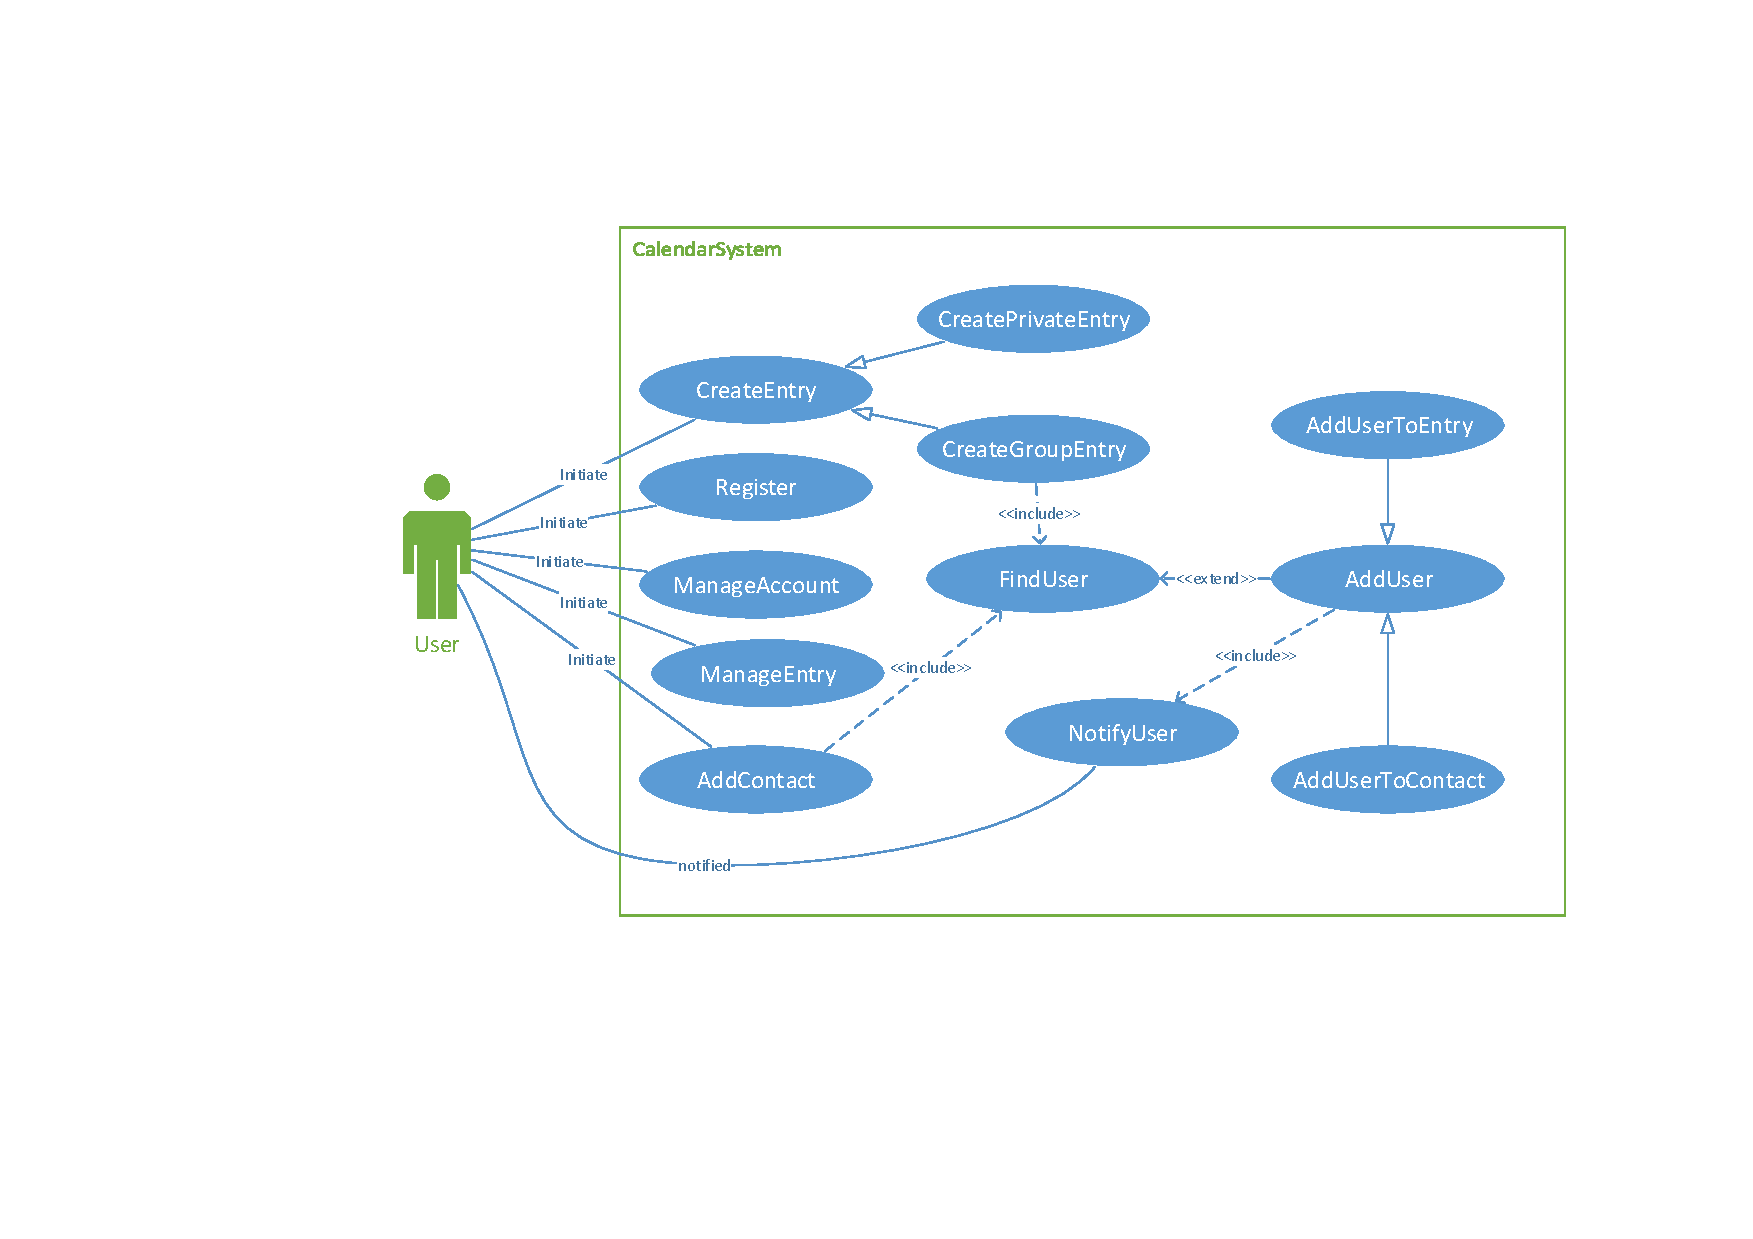
\includegraphics[scale = 0.8]{usecase}
\caption{Use case model}
\end{figure}
\pagebreak
\subsubsection{Use cases}

\begin{center}
    \begin{tabular}{ | l | p{10cm} |}
    \hline
    Use case name & CreateGroupEntry \\ \hline
    Participating actors & Initiated by User - communicates with User \\ \hline
    Flow of events & \tabitem The User creates a GroupEntry \\
    \mbox{} & \tabitem The User searches for other Users and add them to the GroupEntry (Includes the usecases: FindUser and AddUser) \\
    \mbox{} & \tabitem The User confirms input in the entry. \\
    \mbox{} & \tabitem The system confirms entry has been created. \\
    \mbox{} & \tabitem The system sends a notice to all added Users (Includes the use case NotifyUser). \\ \hline
    Entry condition & The User creating the entry is logged in to the CalendarSystem \\ \hline
    Exit condition & Entry has been created \\
	\mbox{} & A notice has been sent to all added Users \\
	\hline
    \end{tabular}
\end{center}

\begin{center}
    \begin{tabular}{ | l | p{10cm} |}
    \hline
    Use case name & AddContact \\ \hline
    Participating actors & Initiated by User - communicates with User \\ \hline
    Flow of events & \tabitem The User opens the AddContact function. \\
    \mbox{} & \tabitem The User searches for the User to add (Includes the use case FindUser). \\
    \mbox{} & \tabitem The User adds the found User, to the ContactList (Includes the use case AddUser). \\
    \mbox{} & \tabitem The system sends a Notice to the added User. \\ \hline
    Entry condition & The User adding another User is logged on \\ \hline
    Exit condition & The Users ContactList contains the added User \\
    \mbox{} & A notice has been sent to the added Users \\
    \hline
    \end{tabular}
\end{center}

\begin{center}
    \begin{tabular}{ | l | p{10cm} |}
    \hline
    Use case name & Register \\ \hline
    Participating actors & Initiated by User \\ \hline
    Flow of events & \tabitem The User opens the register function and plots in any required information. \\
    \mbox{} & \tabitem The User confirms the information and waits for the system. \\
    \mbox{} & \tabitem The system notifies the User that the account has been successfully been created. \\
    \hline
    Entry conditions & The User has installed the Client part of the system \\ \hline
    Exit condition & An account has been created for the User \\
    \hline
    \end{tabular}
\end{center}
\pagebreak
\section{Glossary}


\end{document}